\documentclass[../../main.tex]{subfiles}

% 

\begin{document}
\chapter{Využitie jadrovej fyziky, astrofyzika}

\section{Zadanie}

Aplikácie jadrovej fyziky (jadrová energia, metóda nukleárnej magnetickej rezonancie, Mössbauerov jav, výroba a použitie rádionuklidov, dátovacie metódy atď.), Kozmické žiarenie, Radiačné pásy Zeme, Energia hviezd (protón-protónový cyklus, uhlíko-kyslíkový cyklus), Neutrínová astronómia, Vznik chemických prvkov, Neutrónové hviezdy.

\section{Aplikácie jadrovej fyziky}

\subsection{Jadrová energia}

Jadrová energia alebo nepresne atómová energia je energia uvoľnená pri jadrovej reakcii, presnejšie pri premenách atómových jadier na systémy s absolútne vyššou väzbovou energiou štiepením jadier alebo termojadrovou reakciou. Prejavuje sa okrem iného ako tepelná energia.

Prvý úspešný pokus s jadrovým štiepením vykonali v roku 1938 v Berlíne Otto Hahn, Lise Meitnerová a Fritz Strassmann.

Počas 2. svetovej vojny sa rozbehol jadrový program v rade štátov. Prvá riadená reťazová štiepna reakcia sa uskutočnila 2. decembra 1942 v reaktore CP-1, ktorý pod vedením Enrica Fermiho postavili v podzemí štadiónu Chicagskej univerzity. Motivácia pokusov bola jednak vedecká, ale aj vojenská - reaktory založené na výsledkoch Fermiho výskumu potom slúžili na výrobu plutónia na použitie v jadrovej zbrani. Po zvrhnutí atómových bômb na Hirošimu a Nagasaki sa konštrukcia reaktorov na výrobu plutónia rozbehla aj v ďalších štátoch.

Na výrobu elektriny sa jadrový reaktor prvý raz využil 20. decembra 1951 vo výskumnej stanici EBR-I pri Arce. Zariadenie založené na rýchlom množivom reaktore dodávalo spočiatku výkon okolo 200 kW.

Prvá jadrová elektráreň bola postavená v ZSSR v meste Obninsk. K rozvodnej sieti bola oficiálne pripojená 27. júna 1954. V 5MW reaktore bol použitý grafit ako moderátor a voda ako chladiace médium.

Využitie jadrovej energie sa potom rýchlo rozvíjalo. V roku 1960 tvoril inštalovaný výkon menej ako 1 gigawatt (GW), na konci sedemdesiatych rokov už 100 GW, a 300 GW v osemdesiatych rokoch.

Od konca 80. rokov je nárast oveľa slabší a prevažne tvorený výstavbou jadrových elektrární v Číne. V roku 2005 bol inštalovaný výkon 366 GW. Proti využitiu jadrovej energie sa v niektorých krajinách zdvihla vlna odporu, založená jednak na obavách z nehody (ako napr. Černobyľská havária), jednak na strachu z radiácie. V Rakúsku (1978), Švédsku (1980) a Taliansku (1987) dokonca prebehli referendá, dôsledkom ktorých sa upustilo od využitia jadrovej energie.

Na mierové účely sa v súčasnosti priemyselne využíva štiepná reakcia uránu alebo plutónia, predmetom intenzívneho výskumu je praktické využitie termonukleárnej syntézy vodíka na hélium.

Najvýznamnejším využitím jadrovej energie je výroba elektrickej energie v jadrových elektrárňach. Jadrové zdroje majú dnes približne 17$\%$ podiel na svetovej výrobe elektriny a približne 7$\%$ podiel na spotrebe energie celkovo.

Najväčší podiel elektrického prúdu z jadra dosahuje Litva (asi 80$\%$), Francúzsko (asi 78$\%$) a Belgicko (asi 60$\%$).

Jadrové reaktory sa takisto používajú na pohon lodí a ponoriek, na výrobu izotopov na ďalšie využitie a na výskum, zároveň sa (väčšinou ako vedľajší produkt pri výrobe elektriny) využívajú na vykurovanie či ohrev vody.

Dejiny využitia jadrovej energie poznamenali tri veľké nehody – v roku 1986 v Černobyle, podstatne menšia v roku 1979 v Three Mile Islandu v USA a v roku 2011 v Japonsku v oblasti Fukušima.

\subsection{Nukleárna magnetická rezonancia}

NMR je jav, pri ktorom jadro v magnetickom poli absorbuje a následne emituje elektromagnetické žiarenia. Táto energia má špecifickú rezonančnú frekvenciu ktorá závisí na sile magnetického poľa a na magnetických vlastnostiach izotopu atómu. 

Ak je jadro s nenulovým spinom umiestnené do vonkajšieho magnetického poľa $B_0$, tak toto pole núti magnetický moment jadra zorientovať sa do jeho smeru. Spin jadra však bráni tejto zmene orientácie a výsledkom je, že magnetický moment začne precesovať okolo vonkajšieho poľa, pričom sa jeho orientácia k tomuto poľu nemení - zachováva sa zložka $\mu$ paralelná s $B_0$, zložka $\mu$ kolmá na $B_0$ rotuje v rovine kolmej na $B_0$. Situácia je veľmi podobná k správaniu sa mechanického zotrvačníka v gravitačnom poli.

\begin{figure}[h]
\centering
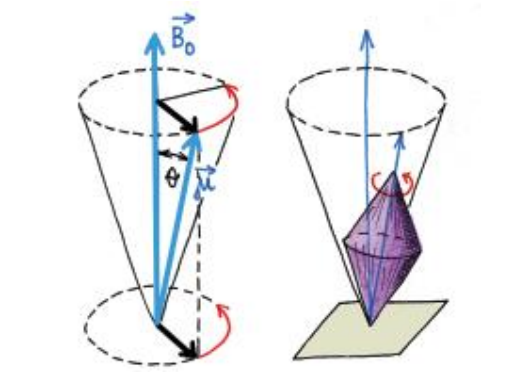
\includegraphics[width=0.4\textwidth]{sf10-nmr.png}
\caption{Precesia atómového magnetického dipólu $\mu$ okolo magnetického poľa $B_0$ a analógia s precesiou mechanického zotrvačníka v gravitačnom poli.}
\label{sf10:img:nmr}
\end{figure}

V NMR sa využívajú magnetické polia $B_0$ s veľkosťou $0,1-20$ T. Pri takýchto poliach je frekvencia precesie spinov v oblasti $1-1000$ MHz, čo je rádiofrekvenčná oblasť.

Všetky vlastnosti atómových jadier závisia od ich zloženia, preto aj NMR vlastnosti sú pre každý izotop iné. Znamená to, že rôzne izotopy toho istéhu prvku majú iné NMR vlastnosti. Niektoré dôležité, v prírode bohato zastúpené izotopy ($^{12}$C, $^{16}$O) majú spin aj magnetický moment nulový a preto sú v NMR neaktívne. Pre organickú chémiu a biochémiu sú najdôležitejšími jadrami vodík (izotop $^1$H, výskyt $99,98\%$) a uhlík (izotop $^{13}$C, výskyt $1,1\%$).

Merateľnou veličinou v NMR je výsledný magnetický moment všetkých spinov vo vzorke, ktorý sa nazýva magnetizácia vzorky $M$. Ak je vzorka mimo magnetického poľa, tak všetky orientácie individuálnych atómových magnetických momentov sú pravdepodobne rovnaké a výsledná magnetizácia je nulová. Ak sa vzorka vloží do silného magnetického poľa, tak podľa zákonov termodynamiky budú orientácie viac paralelné s poľom $B_0$ energeticky výhodnejšie a preto v rovnovážnej vzorke aj viac zastúpené.

Ak sa na vzorku v rovnováhe aplikuje elektromagnetické žiarenia, ktoré má rovnakú frekvenciu, ako je precesia spinov $f_0$, vychýli sa magnetizácia zo smeru $B_0$ a vznikne nerovnovážna magnetizácia $M$, ktorá precesuje okolo $B_0$ podobne ako každý individuálny spin. Takáto magnetizácia je dobre merateľná a je tou veličinou, ktorá sa pri NMR experimentoch priamo meria. 

Z uvedeného vyplýva schéma základného NMR experimentu. Na začiatku experimentu sa vzorka nechá voľne relaxovať, pričom nastáva jej polarizácia. Vytvorí sa rovnovážna magnetizácia, ktorá sa potom krátkym pôsobením elektromagnetického žiarenia preklopí do roviny kolmej na $B_0$. Vzniknutá nerovnovážna magnetizácia precesuje okolo $B_0$ a indukuje v cievke prijímača signál, ktorý sa digitalizuje a ukladá do pamäti počítača. 

\subsection{Výroba a využitie rádionuklidov}

Rádionuklid alebo rádioaktívny nuklid je atóm, ktorého jadro sa samovoľne premieňa za vysielania vysokoenergetického žiarenia. V dnešnej dobe sa pre potreby nukleárnej medicíny používajú iba umelo pripravené rádionuklidy, ktoré dosahujú vysoké čistoty. Získavajú sa z:

\begin{itemize}
\item cyklotrónov ($^{111}$In, $^{123}$I, $^{201}$Tl)

Kladne nabité častice sú urýchľované a narazia do terča, vyrobeného z materských prvkov. Jadrovými interakciami sa mení ich jadrová štruktúra a protónové čísla. Po ožarovaní sa z terča chemickými reakciami uvoľní rádionuklid.

\item jadrových reaktorov ($^{99}$Mo, $^{59}$Fe)

Z jadrových reaktorov štiepiacich $^{235}$U možno získavať jednak rádioizotopy izoláciou zo štiepnych produktov, jednak možno využiť vzniknuté neutróny. 

\item rádionuklidových generátorov ($^{99m}$Tc, $^{81m}$Kr, $^{68}$Ga, $^{90}$Y)

Vďaka svojej cene, veľkosti, jednoduchosti a ľahkému použitiu sú najpoužívanejším zdrojom rádionuklidov.
\end{itemize}

Rádionuklidy sa používajú v mnohých odvetviach, a to napr.
\begin{itemize}
\item strojárenstvo a technika
\begin{itemize}
\item Zisťovanie skrytých vád materiálu (bezdotykové meranie hrúbky materiálu) - využíva sa zoslabenie žiarenia pri prechode látkou
\item Konštrukcia termočlánkov na výrobu elektriny - využíva sa Seebeckov jav a teplo uvoľnené pri rádioaktívnej premene
\end{itemize}
\item medicína a lekárstvo
\begin{itemize}
\item Liečenie zhubných nádorov
\item Sledovanie prietoku krvi - rádionuklid $^{99m}$Tc ako žiarič $\gamma$ s polčasom premeny 6 hodín
\item Zisťovanie činnosti štítnej žľazy - $^{132}$I s polčasom premeny 2 hodiny
\item Liečba reumatických chorôb
\item Výroba liečiv
\item Sterilizácia lekárskych nástrojov a predmetov
\end{itemize}
\item archeológia a geológia
\begin{itemize}
\item Meranie veku hornín zemskej kôry
\item Zisťovanie veku rôznych vykopávok
\end{itemize}
\item ochrana životného prostredia
\begin{itemize}
\item Detektory dymu
\item Hlásiče požiaru
\item Sledujú rozptyl škodlivých a prítomnosť toxických látok
\end{itemize}
\item potravinárstvo
\begin{itemize}
\item Ošetrenie potravín (zabraňuje sa ich skazeniu alebo klíčeniu)
\end{itemize}
\end{itemize}

\subsection{Dátovacie metódy}

Rádioaktívne datovanie je technika používaná na datovanie materiálov, obvykle založená na porovnávaní medzi množstvom prirodzene sa vyskytujúceho rádioaktívneho izotopu s produktami jeho rozpadu. Je to jeden z hlavných informačných prameňov o veku hornín, veku Zeme a podobne. Využíva sa na datovanie širokého okruhu prírodných aj umelých materiálov. Najznámejšou technikou je rádiouhlíkové datovanie. Existujú aj ďalšie, ako napr. draselnoargónové datovanie a uránové datovanie. Poskytuje významný informačný prameň o veku fosílií a o pomeroch na zemi behom jej evolúcie.

Rádiouhlíková metóda datovania je založená na výpočtu veku z poklesu počtu atómov izotopu $^{14}$C v pôvodne živých objektoch. Táto metóda bola objavená v roku 1940 a používa sa hlavne v archeológii, ale aj v etnobotanických vedách.

Uhlík sa využíva preto, že je z veľkej časti zastúpený v každom živom organizme. V prírode sa izotop $^{14}$C vyskytuje ako $0,0000000001\%$ všetkého uhlíku. Zároveň však v živých organizmoch, rovnako ako kdekoľvek inde, dochádza k jeho rozpadu. Zmeraním pomeru jeho koncentrácie k stabilnému $^{12}$C je potom možné vypočítať dobu, kedy bola vzorka vyradená z kolobehu v prírode (kedy organizmus zomrel).

Podrobnejšie vychádza princíp rádiouhlíkového datovania z faktu, že sa v atmosfére zachováva rovnováha medzi tvorbou $^{14}$C dopadom kozmického žiarenia a jeho prirodzeným rádioaktívnym rozpadom. Tým pádom panuje aj rovnováha medzi koncentráciami $^{14}$C a ostatných izotopov uhlíka. Pomer týchto koncentrácií je teda v čase konštantný a to platí aj pre uhlík, ktorý sa dostane do tela živých organizmov. Táto situácia trvá do tej doby, než organizmus zomrie. Do mŕtveho tela už nový uhlík nevstupuje, no izotop $^{14}$C sa naďalej rozpadá.

Na dlhšie časové úseky sa používa argón a urán, pretože koncentrácia $^{14}$C sú už príliš nízke, než aby mohli byť ich rozdiely zmerané.

\section{Kozmické žiarenie}

Kozmickým žiarením sa nazýva žiarenie, ktoré dopadá na Zem z kozmického priestoru. Štúdium kozmického žiarenia zohralo v minulosti dôležitú úlohu pri vzniku fyziky elementárnych častíc, keďže prvé elementárne častice boli objavené práve pri tomto štúdiu. Bol to pozitrón, mión, pión a ďalšie, ktoré sa podarilo objaviť v tridsiatych až päťdesiatych rokoch.

V tej dobe predstavovalo žiarenie prichádzajúce z vesmíru prakticky jediný zdroj častíc s vyššími energiami, ako poskytovali rádioaktívne rozpady a vtedajšie urýchľovače. Častice kozmického žiarenia dosahujú síce až energie $10^{20}$ eV, ale len s veľmi malou početnosťou. 

Fyzika kozmického žiarenia má uplatnenie v geofyzike, astrofyzike a v kozmológii.

\subsection{Primárne kozmické žiarenia}

Kozmické žiarenie, ktoré sa pozoruje za hranicami zemskej atmosféry, sa nazýva primárne kozmické žiarenie. Medzi jeho základné vlastnosti patrí časovo nemenná hustota toku a izotropný dopad na vonkajšie vrstvy atmosféry. Celková intenzita zo všetkých smerov tvorí približne $0,7-1$ častíc na $\unit{s\cdot cm^2}$. Maximálne energie dopadajúcich častíc je $10^{19}$ eV, zatiaľčo stredná energia je zhruba GeV.

Primárne kozmické žiarenie sa skladá prevažne z protónov (90$\%$), deuterónov (7$\%$), $\alpha$ častíc ($1\%$), elektrón-pozitrónových párov ($1\%$) a jadier ľahkých prvkov ($1\%$). S rastúcou energiou častíc rastie relatívne zastúpenie prvkov s veľkým $Z$ a klesá relatívne zastúpenie protónov.

Minimálna energia nabitej častice primárneho žiarenia, ktorá ešte môže dopadnúť na povrch Zeme, závisí na zemepisnej šírke vzťahom 
\begin{equation}
E\approx 1,9\cdot 10^{10} \cos^4(\varphi)\:\unit{eV}
\end{equation}

Nabitá častica nalietavajúca do magnetického poľa Zeme sa pohybuje po špirále pozdĺž siločiar magnetického poľa Zeme smerom k pólom. Preto je intenzita kozmického žiarenia na póloch väčšia, než na rovníku - tento efekt sa nazýva šírkový efekt. Okrem toho sa pozoruje tzv. \textit{východo-západná anomália}. Intenzita kozmického žiarenia prichádzajúceho zo západného zmeru je väčšia, než z východného smeru, čo súvisí s tým, že väčšina častíc primárneho kozmického žiarenia je kladne nabitá.

Častice primárneho kozmického žiarenia, ktoré vstupujú do atmosféry Zeme, sa zrážajú s atómami a jadrami a interagujú s nimi. Pri týchto interakciách sú z atómových obalov vyžiarené elektróny a z jadier nukleóny a vznikajú aj ďalšie častice. Absorpciou primárneho kozmického žiarenia s jednak predáva energia ionizáciou do atmosféry a tak vzniká veľký počet častíc sekundárneho kozmického žiarenia.

\subsection{Sekundárne kozmické žiarenie}

Sekundárne kozmické žiarenie delíme dvomi spôsobmi - podľa prenikavosti v látkach a podľa jeho zloženia.

Keď meriame intenzitu sekundárneho kozmického žiarenia pred prechodom látkou a po ňom, pozorujeme najskôr rýchly pokles hustoty toku prejdeného žiarenia s rastúcou hrúbkou látky. Po dosiahnutí istej kritickej hodnoty sa pokles podstatne zmierni. Tento fakt viedol k rozdeleniu kozmického žiarenia podľa prenikavosti. Sekundárne žiarenie teda delíme na dve zložky - mäkkú, ktorá sa v látkach silno pohlcuje, a tvrdú (prenikavú), ktorá sa v látkach naopak pohlcuje slabo. Mäkkú zložku tvoria predovšetkým nízkoenergetické protóny, pióny a elektrón-fotónový komponent. Oproti tomu prenikavú zložku tvoria hlavne vysokoenergetické mióny a jadrový aktívny komponent.

Aby sme vysvetlili druhý spôsob triedenia, preberieme podrobnejšie interakciu primárneho vysokoenergetického protónu s látkou v zemskej atmosfére. Protón bude strácať energiu od vstupu do atmosféry zrážkami s elektrónmi v obaloch atómov, pri ktorých sa budú atómy ionizovať, a zrážkami s atómovými jadrami. Pri zrážke protónu s jadrami vznikajú okrem veľkého množstva nabitých častíc tiež neutrálne častice, napr. neutróny či $\pi^0$ mezóny. Neutróny, potom čo sa dostatočne spomalia zrážkami s jadrami, sú absorbované jadrami dusíku (n+$^{14}_7$N$\rightarrow ^{14}_6$C+p). Mezóny sa však rozpadajú na dva fotóny
\begin{equation}
\pi^0\rightarrow \gamma + \gamma
\end{equation}
a tieto fotóny vytvárajú počiatok tzv. elektromagnetickej kaskády. V poli atómových jadier produkujú páry elektrónu a pozitrónu, pričom elektrón aj pozitrón vylietavajú prevažne pod malými uhlami vzhľadom ku smeru letu pôvodného fotónu. Pohybujúci sa elektrón aj pozitrón môžu vyžiariť v poli jadra brzdný fotón, ktorý opäť vytvára pár $e^-e^+$, a tak ďalej.

 Vzhľadom k tomu, že pri brzdnom žiarení a pri tvorbe páru sa energia s veľkou pravdepodobnosťou rozdelí na dve približne rovnako veľké časti, zmenšovanie energie v kaskáde prebieha exponenciálne a počet častíc rastie lavínovito až do tej doby, než energia jednotlivých častíc klesne natoľko, že sa častice začnú pohlcovať v obaloch atómov či molekúl. V elektromagnetickej kaskáde sú produkované častice kolimované prevažne do pôvodného smeru častice vyvolávajúcej kaskádu.
 
 Počet častíc v kaskáde závisí na energii primárnej častice. Pre energie častíc $\sim 10^{15}$ eV možno zaznamenať detektormi na zemskom povrchu častice z kaskády vyvolané jednou primárnou časticou až na rozlohe niekoľko stoviek metrov štvorcových. Nemožno ale prakticky rozlíšiť, aká primárna častica kaskádu vyvolala.
 
Sekundárne kozmické žiarenie tak podľa zloženia delíme na:
\begin{itemize}
\item \textbf{elektrón-fotónová zložka} - sem patria fotóny, elektróny a pozitróny, ktoré sú zložkami elektromagnetickej kaskády a sú tiež súčasťou mäkkej zložky žiarenia
\item \textbf{jadrová aktívna zložka} - podobne ako elektromagnetická kaskáda sa vytvárajú aj spŕšky iného typu. Sú vyvolané nukleónmi a nabitými piónmi a spŕška tohto druhu je vytváraná hlavne silnými interakciami častíc. Aj táto spŕška postupuje v úzkom kuželi a vyvíja sa tak dlho, dokým energia častíc neklesne na niekoľko desiatok MeV.
\item \textbf{miónová zložka} - na úrovni mora už väčšina častíc sekundárneho kozmického žiarenia nepatrí ani k jednej z predchádzajúcich zložiek. Väčšinu častíc v nej tvoria mióny, ktoré vznikli rozpadom $\pi^\pm$ ($\pi^+\rightarrow\mu^++\nu_\mu$ a $\pi^-\rightarrow\mu^-+\bar{\nu}_\mu$) a ktoré majú strednú dobu života $\tau_\mu\sim 10^{-6}$ s. Vzhľadom k tomu, že mióny interagujú s látkou elektromagneticky a slabo, nielenže sa dostanú na úroveň mora, ale môžu preniknúť aj do veľkých hĺbok pod povrch Zeme. 
\end{itemize}

\subsection{Pôvod kozmického žiarenia}

Výskum zloženia primárnej zložky kozmického žiarenia môže dať odpoveď na otázku, odkiaľ kozmické žiarenia pochádza a akým spôsobom získavajú častice energie dosahujúce $10^{20}$ eV.

\begin{figure}[h]
\centering
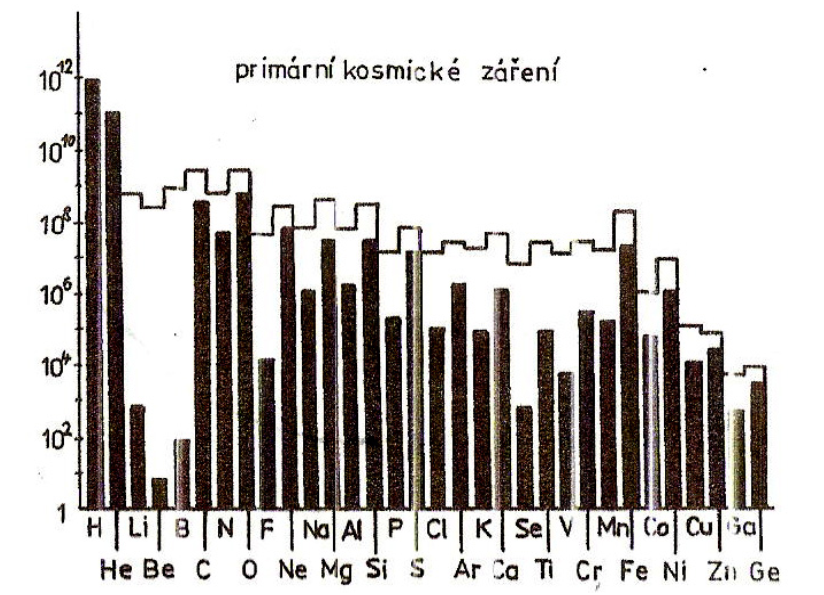
\includegraphics[width=0.6\textwidth]{sf10-prvky.png}
\caption{Relatívne zastúpenie prvkov v primárnej zložke kozmického žiarenia so strednou energiou $4$ GeV/nukleón (biely histogram) v porovnaní so zastúpením prvkov v galaxii (čierny histogram).}
\label{sf10:img:prvky}
\end{figure}

Na obrázku \ref{sf10:img:prvky} je uvedené zastúpenie prvkov s atómovým číslom $1\leq Z\leq 32$ obsiahnutých v kozmickom žiarení a je porovnané so zastúpením prvkov v galaxii určeným zo spektrálnych meraní a z analýzy meteoritov.

Obe zastúpenia vykazujú síce dosť značné rozdiely, napr. výskyt ťažkých prvkov je v kozmickom žiarení väčší než v galaktickej hmote a tiež variancie v závislosti na $Z$ vo výskyte prvkov v kozmickom žiarení sú menšie než pre hmotu v galaxii. Rozdiel však nie je tak drastický, aby nemohol byť vysvetlený napr. tým, že ťažké nuklidy v kozmickom žiarení sa rozpadli pod vplyvom interakcie s medzihviezdnou hmotou na ľahšie.

Toto porovnanie vylučuje niektoré hypotézy o pôvode kozmického žiarenia:
\begin{itemize}
\item Je v rozpore s hypotézou, že kozmické žiarenie vzniklo pri Veľkom tresku. Pri ňom by sa mal prakticky výlučne produkovať vodík a tým pádom by kozmické žiarenie nemohlo obsahovať ťažšie prvky.

\item Rovnako nie je v súlade s hypotézou, že kozmické žiarenie vzniklo zo starých hviezd, pretože potom by podiel ťažkých prvkov musel byť väčší, než sa pozoruje.

\item Štúdium stôp zanechaných ionizujúcim kozmickým žiarením v kryštalickej stavbe meteoritov naznačuje, že kozmické žiarenie nevzniklo ani behom lokálnej katastrofy (výbuch supernovy). Hustota kozmického žiarenia v Slnečnej sústave totiž zostáva konštantné po celú poslednú miliardu rokov.

\item Oproti tomu existujú aj hypotézy, ktoré nie sú v tak silnom rozpore s uvedenými dátami, ale ktoré popisujú iba častice s energiou neprekračujúcou 10 GeV. Jedna z nich hľadá pôvod kozmického žiarenia v Slnečnej sústave a za jeho zdroj považuje slnečné škvrny, z ktorých sú vysielané behom zvýšenej slnečnej aktivity nabité častice, ktoré sú urýchľované magnetickým poľom Slnka.

\item Inú hypotézu navrhol Enrico Fermi. Častice sa podľa nej pri zrážkach s medzihviezdnou hmotou urýchľuje alebo spomaľuje a vďaka štatistickým fluktuáciám urýchlenie môže nadobudnúť až exponenciálneho charakteru v závislosti na počte zrážok alebo veku častice. Bohužiaľ sa táto hypotéza nehodí pre urýchľovanie ťažkých častíc a je v rozpore s údajmi o rýchlosti medzihviezdnych mračien, ktorá je rádovo rovná 10 km/s, a je preto na urýchľovanie Fermiho mechanizmom nepostačujúca.
\end{itemize}

Po objave nových astronomických objektov, ako sú pulzary, s magnetickými poľami o mnoho rádov intenzívnejšími, než je magnetické pole Zeme, prevládla hypotéza, že častice nezískavajú energiu spojito, ale pulzne v pulzaroch alebo počas výbuchu supernov. Ani tieto zdroje nestačia na to, aby vysvetlili existenciu kozmického žiarenia s najvyššími energiami. Je preto možné, že najenergetickejšia zložka kozmického žiarenia vzniká za hranicami našej galaxie.

\subsection{Detekcia kozmického žiarenia}

Snahy o kvantitatívnu registráciu kozmického žiarenia mali značný význam pre detekciu elementárnych častíc vôbec.

Častice primárneho kozmického žiarenia sa registrujú vo veľkých výškach nad povrchom Zeme detektormi umiestnenými v balónoch alebo na umelých družiciach Zeme. S pomocou družíc a balónov nie je však možné efektívne registrovať častice s veľmi vysokými energiami, pretože rozmery detektoru pre tento účel sú podstatne väčšie, než veľkosť nosného zariadenia. Preto sa stále budujú laboratória kozmického žiarenia vo vysokohorských oblastiach.

Jadrá prvkov a protóny primárneho kozmického žiarenia, ako ukazuje pozorovanie, dopadajú do atmosféry Zeme prakticky izotropne. To ale nemusí byť dané tým, že zdroje kozmického žiarenia sú rozložené izotropne, ale tým, že okrem magnetického poľa Zeme pôsobí na nabité častice ešte magnetické pole galaxie, ktoré dráhy častíc deformuje, takže častice sa pohybujú priestorom po špirálach, a preto sa zobrazenie prípadného zdroja rozmazáva.

Jedinými vhodnými kandidátmi na skúmanie možných zdrojov kozmického žiarenia sú preto neutrálne častice bez elektrického náboja. Z nich ale neprichádzajú do úvahy neutróny, pretože sa rozpadajú $\beta$ rozpadom ešte skôr, ako dopadnú na Zem. V $\beta$ rozpade vznikajúce antineutrína sú častice interagujúce slabo a boli by vhodnými kandidátmi, keby nebolo tak obtiažne ich registrovať.

Na zmapovanie možných zdrojov kozmického žiarenia preto možno prakticky použiť $\gamma$ žiarenie. Môžeme totiž očakávať, že pri urýchľovaní nabitých častíc kozmického žiarenia až na energie $10^{20}$ eV dochádza k vyžarovaniu vysokoenergetických fotónov s energiami rovnakého rádu.

Fotóny kozmického žiarenia nie je možné detekovať priamo na úrovni morskej hladiny, pretože pri prelete atmosférou interagujú s atómami a vytvárajú elektromagnetické kaskády. Môžu síce byť zaznamenané v družiciach, ale iba do určitej energie. Rozmery družíc neumožňujú totiž detekovať toky fotónov menšie než 1 fotón m$^{-2}$ za mesiac.

K detekcii primárnych fotónov sa používajú dve metódy: v jednej sa zaznamenávajú priamo sekundárne častice elektromagnetickej kaskády detektormi umiestnenými na sústredných kružniciach na ploche niekoľko stoviek m$^2$. Táto metóda je vhodná pre fotóny s energiami $>10^{15}$ eV. V druhej metóde sa detekuje Čerenkovovo žiarenie vysielané nabitými časticami elektromagnetickej kaskády, a to aj v prípade, že tieto častice na Zem nedopadnú, ale absorbujú sa v atmosfére. Táto metóda umožňuje znížiť energetický prah detekcie až do $10^{12}$ eV. Pozorovanie Čerenkovovho žiarenia sa robí za bezmesačných nocí teleskopom zloženým zo zrkadiel, ktorý fokusuje svetlo do fotonásobiča.

Ani jedna z uvedených metód však nemôže stanoviť, či primárnou časticou bol vysokoenergetický fotón alebo nejaká nabitá častica, ktorých rozloženie by malo byť izotropné. To vedie k nutnosti študovať na pozadí izotropného žiarenia z vesmíru anizotropie elektromagnetických kaskád prichádzajúcich z daného smeru.

Jedným zo závažných problémov fyziky kozmického žiarenia je tiež detekcia slnečných neutrín. K výskumu neutrínovej zložky kozmického žiarenia sa budujú laboratória vo veľkých hĺbkach pod povrchom zeme, aby boli odfiltrované ostatné zložky kozmického žiarenia.


\section{Radiačné pásy zeme}

Pre nabité častice s energiami menšími než približne 1 GeV existujú v magnetickom poli Zeme pasce, z ktorých sa nemôžu dostať von. Tieto magnetické pasce majú tvar toroidov a obklopujú Zem v šírkovom smere. Ich vzdialenosť od povrchu Zeme je určená energiou častíc. Čím je energia vyššia, tým bližšie k Zemi sa pasca nachádza. Tieto pasce potom tvoria prirodzený rezervoár nabitých častíc.

Existenciu týchto pásov vedci teoreticky predpokladali už v dobe pred kozmickou érou. Potvrdili ich až merania družíc Explorer I (v roku 1958) a neskôr aj Explorer III, o ktoré sa zaslúžil James Van Allen, po ktorom sú pásy pomenované.

Oblasti žiarenia si môžeme predstaviť ako vnútorný a vonkajší pás obopínajúci Zem. Vnútorný pás sa skladá prevažne z protónov, zatiaľčo vonkajší pás tvoria najmä elektróny. Častice v týchto pásoch dokáže preniknúť oloveným štítom s hrúbkou 1 mm.

Termín Van Allenove pásy súvisí z radiačnými pásmi okolo Zeme, ale podobné pásy boli objavené aj okolo ďalších planét. Kvôli zemskej atmosfére sa pri našej planéte vyskytujú až vo výške 200 až 1000 km. Pásy končia pri uhle 65$^\circ$ pod rovníkom, priamo nad pólmi sa nenachádzajú.

\begin{figure}[h]
\centering
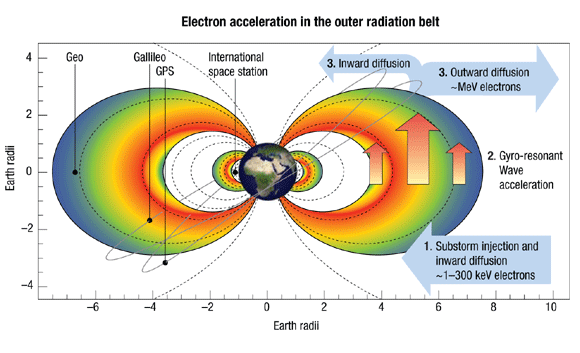
\includegraphics[width=0.8\textwidth]{sf10-vanallen.png}
\caption{Van Allenove radiačné pásy.}
\label{sf10:img:vanallen}
\end{figure}

\subsection{Vonkajší (elektrónový) Van Allenov pás}

Veľký vonkajší pás radiácie sa nachádza vo výške od 13 do 60 tisíc kilometrov, najintenzívnejšie vo výške 14,5 až 19 tisíc km. Vedci sa domnievajú, že ho tvorí plazma zachytená magnetosférou Zeme. Bolo namerané, že sa v páse nachádza len malé množstvo častíc nabitých vysokou energiou.

Prítomnosť častíc vo vonkajšom páse je rôzna, primárne sa tu ale vyskytujú elektróny a rôzne ióny. Väčšina iónov je vo forme energetických protónov, ale určité percento tvoria aj $\alpha$ častice a kladné ióny kyslíku. Táto zmes iónov naznačuje, že častice obsiahnuté vo vonkajšom páse pravdepodobne pochádzajú z viacerých rôznych zdrojov. Prítomné elektróny tu prúdia rýchlo pozdĺž vonkajšieho okraja pásu, nadobúdajú pritom kinetických energií 40 až 100 keV a ich stredné doby života sú v rozmedzí $10^5$ až $10^7$ s.

Vonkajší pás je väčší a rozptýlenejší ako vnútorný, častice v ňom sú premenlivejšie a mávajú nižšie kinetické energie.

\subsection{Vnútorný (protónový) Van Allenov pás}

Vnútorný pás sa rozkladá zhruba vo výške 1 až 6 tisíc km nad povrchom Zeme. Obsahuje vysoké koncentrácie energetických protónov, zachytených silným magnetickým poľom, s energiami od 20 do 800 MeV a so strednou dobou života približne 100 rokov.

Medzi vedcami panuje domnienka, že protóny s energiami väčšími, než 50 MeV v nižších výškach sú dôsledkom $\beta$ rozpadu neutrónov kozmického žiarenia. Zdrojom protónov s nižšími energiami je pravdepodobne difúzia protónov závislá na zmenách v magnetickom poli v priebehu geomagnetických búrok.

\section{Jadrové procesy v hviezdach}

Na to aby sa teleso dalo charakterizovať ako hviezda, musia v jeho vnútri prebiehať termojadrové reakcie alebo muselo fázou termojadrových reakcií prejsť v minulosti. Termojadrová reakcia je reakcia, pri ktorej sa jadrá atómov ľahkých chemických prvkov zlúčia za vzniku ťažšieho prvku. Keďže jadrá atómov sú kladne nabité a navzájom sa silne odpudzujú, na spustenie termojadrovej reakcie je potrebná veľmi vysoká teplota a tlak, ktoré tieto odpudivé sily prekonajú.

U veľkej väčšiny hviezd (tzv. hlavnej postupnosti) vstupujú do reakcie jadrá najľahšieho známeho chemického prvku vodíka a výsledným produktom je hélium. Premena ľahkého vodíka na hélium môže prebiehať dvoma odlišnými spôsobmi a to protón-protónovým cyklom alebo uhlíkovo-dusíkovo-kyslíkovým cyklom (nazývaným aj CNO cyklus podľa chemických značiek prvkov, ktoré sa ho zúčastňujú). Na to, ktorý z týchto cyklov v jadre hviezdy prevláda, má vplyv hlavne teplota v jadre. Do 16 miliónov stupňov je dominantný protón-protónový cyklus, nad touto hranicou prevláda CNO cyklus. Pre fungovanie CNO cyklu je nevyhnutná tiež prítomnosť týchto troch prvkov v jadre hviezdy. Čistá váha novovzniknutého atómového jadra v termojadrovej reakcii je menšia ako súčet hmotností pôvodných jadier. Pri obidvoch cykloch sa zhruba 1/140 hmoty premení na čistú energiu v súlade s Einsteinovou rovnicou $E = mc^2$. Proces fúzie vodíka je veľmi citlivý na teplotu, takže aj mierne zvýšenie teploty jadra spôsobí značný nárast v rýchlosti fúzie. Preto sú teploty v jadrách hviezd hlavnej postupnosti v rozpätí od 4 miliónov kelvinov pre malé hviezdy triedy M po 40 miliónov kelvinov pri ťažkých hviezdach triedy O.

\subsection{Protón-protónový cyklus}

V Slnku, pri teplote 10 miliónov kelvinov, prebieha fúzia vodíka protónovo-protónovým cyklom:
\begin{subequations}
\begin{equation}
4^1\mathrm{H}\rightarrow2^2\mathrm{H}+2e^+2+2\nu_e \:\:(4,0\:\unit{MeV}+1,0\:\unit{MeV})
\end{equation}
\begin{equation}
2^1\mathrm{H}+2^2\mathrm{H}\rightarrow 2^3\mathrm{He}+2\gamma \:\:(5,5\:\unit{MeV})
\end{equation}
\begin{equation}
2^3\mathrm{He}\rightarrow ^4\mathrm{He}+2^1\mathrm{H} \:\:(12,9\:\unit{MeV})
\end{equation}
\end{subequations}

Sumárom týchto reakcií je:
\begin{equation}
4^1\mathrm{H}\rightarrow ^4\mathrm{He}+2e^++2\gamma+2\nu_e \:\:(26,7\:\unit{MeV})
\end{equation}
kde $e^+$ je pozitrón, $\gamma$ je fotón gama žiarenia, $\nu_e$ je neutríno a H a He sú izotopy vodíka a hélia. Energia uvoľnená v tejto reakcii je rádovo v miliónoch elektrónvoltov, to je len maličké množstvo energie. Keďže však neustále prebieha obrovské množstvo týchto reakcií, množstvo energie je dostatočné na udržanie výstupu žiarenia hviezdy.

\begin{figure}[h]
\centering
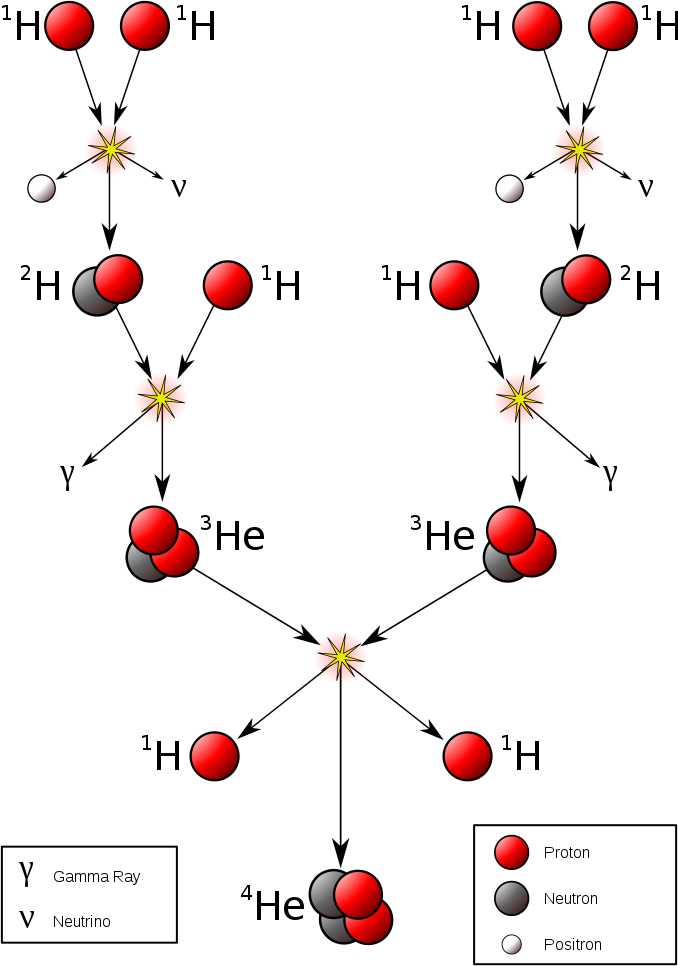
\includegraphics[width=0.4\textwidth]{sf10-pp.png}
\caption{Schéma priebehu protón-protónového cyklu.}
\label{sf10:img:pp}
\end{figure}

\subsection{CNO cyklus}

Uhlíkový cyklus, uhlíkovo-dusíkovo-kyslíkový cyklus, CNO cyklus alebo Betheho-Weizsäckerov cyklus je cyklus jadrových reakcií, pri ktorých sa za účasti uhlíka C, dusíka N a kyslíka O premenia v konečnom dôsledku jadrá vodíka H na jadrá hélia He. Uhlíkový cyklus je základným zdrojom žiarivej energie hviezd s hmotnosťou presahujúcou hmotnosť Slnka. Prebieha postupne nasledujúcimi čiast­kovými reakciam:

\begin{subequations}
\begin{equation}
^{12}\mathrm{C}+^1\mathrm{H}\rightarrow ^{13}\mathrm{N}+\gamma\:\:(1,94\:\unit{MeV})
\end{equation}
\begin{equation}
^{13}\mathrm{N}\rightarrow ^{13}\mathrm{C}+e^++\nu_e\:\:(2,22\:\unit{MeV})
\end{equation}
\begin{equation}
^{13}\mathrm{C}+^1\mathrm{H}\rightarrow ^{14}\mathrm{N}+\gamma\:\:(7,55\:\unit{MeV})
\end{equation}
\begin{equation}
^{14}\mathrm{N}+^1\mathrm{H}\rightarrow ^{15}\mathrm{O}+\gamma\:\:(7,30\:\unit{MeV})
\end{equation}
\begin{equation}
^{15}\mathrm{O}\rightarrow ^{15}\mathrm{N}+e^++\nu_e\:\:(2,76\:\unit{MeV})
\end{equation}
\begin{equation}
^{15}\mathrm{N}+^1\mathrm{H}\rightarrow ^{12}\mathrm{C}+^4\mathrm{He}\:\:(4,97\:\unit{MeV})
\end{equation}
\end{subequations}

Celkové množstvo energie, ktoré sa uvoľní pri vzniku jedného jadra hélia vo forme $\gamma$ žiarenia je 26,74 MeV ($4,284\cdot 10^{-12}$ J), zvyšok energie sa uvoľní vo forme neutrín $\nu_e$. Cyklus sa uplatňuje v centrálnych oblastiach hviezd pri teplotách 16-50 mil. K

\begin{figure}[h]
\centering
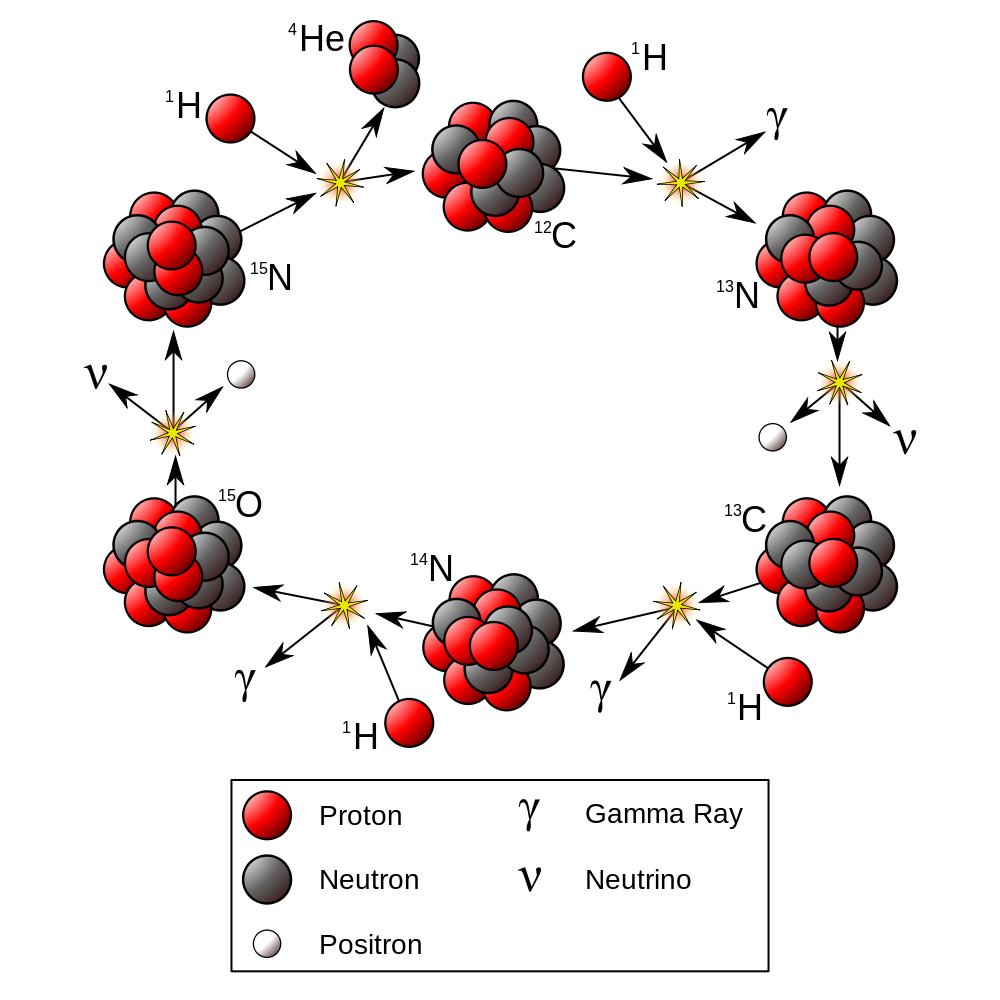
\includegraphics[width=0.6\textwidth]{sf10-cno.png}
\caption{Schéma priebehu CNO cyklu.}
\label{sf10:img:cno}
\end{figure}

\section{Neutrínová astronómia}

Neutrínová astronómia je oblasť astronómie, ktorá sa zaoberá výskumom neutrín kozmického pôvodu. V kozmických podmienkach vznikajú neutrína pri termonukleárnych reakciách v Slnku a vo hviezdach, najmä pri vzplanutiach supernov. Veľký počet neutrín musel vzniknúť v začiatočných fázach vývoja vesmíru (reliktové neutrína s terajšou teplotou okolo 2 K). Pri súčasných pozorovacích možnostiach sa dajú registrovať iba neutrína slnečného pôvodu. Pravdepodobnosť registrovania neutrín je veľmi nízka, lebo neutrína extrémne slabo reagujú s inými časticami (prúd neutrín môže prejsť bez poznateľného poklesu cez mnoho miliónov hviezd). Na zvýšenie pravdepodobnosti registrovania slnečných neutrín sa používa neutrínový ďalekohľad. Prvé zariadenie tohto typu pozostávalo z veľkého tanku s obsahom 400 m$^3$, naplneného tetrachlóretylénom C$_2$Cl$_4$. Tank bol umiestený v šachte hlboko pod povrchom Zeme (1 500 m), aby sa vylúčil vplyv kozmického žiarenia. Pri reakcii neutrín s atómami chlóru vznikajú rádioaktívne atómy argónu, ktorých prítomnosť možno zistiť; ich počet za jednotku času udáva počet reagujúcich neutrín. Obdobne možno využiť na registráciu toku neutrín vyvolané jadrové reakcie s premenou lítia na berýlium alebo gália na germánium. Uskutočnené experimenty registrovali prekvapujúco nízky tok slnečných neutrín, okolo 1 SNU namiesto teoreticky očakávaného toku okolo 7,5 SNU; táto diferencia nie je dosiaľ spoľahlivo objasnená.

\section{Vznik chemických prvkov}

Pri veľkom tresku vznikli dva prvky - vodík a hélium. Od tej doby vznikajú ďalšie prvky v jadrách hviezd a pri výbuchoch hviezd. Práve prostredníctvom hviezdnych výbuchov sa tieto ďalšie prvky rozptyľujú do medzihviezdneho priestoru a stávajú sa súčasťou novo vznikajúcich hviezd a planét.

Celkovo prebiehajú tieto procesy syntézy ľahších prvkov:
\begin{itemize}
\item $^4$He vzniká spaľovaním vodíku
\item $^3$He vzniká pri nedokončenej protón-protónovej reakcii
\item Li, Be a B sú pri teplotách jadier hviezd nestabilné a tým možno vysvetliť ich relatívne nízke zastúpenie vo vesmíre. Ich atómy boli vytvorené buď syntézou v období veľkého tresku alebo vznikli rozpadom ťažkých jadier v medzihviezdnom priestore pri dopade kozmického žiarenia.
\item $^{12}$C, $^{16}$O, $^{18}$O, $^{22}$Ne vznikajú pri spaľovaní hélia
\item $^{14}$N, $^{13}$C, $^{15}$N, $^{17}$O sú produkty neukončeného CNO cyklu
\item $^{20}$Ne, $^{24}$Mg, $^{26}$Al, $^{28}$Si, $^{30}$P, $^{32}$S vznikajú spaľovaním uhlíku
\end{itemize}

Všeobecne možno povedať, že behom života hviezdy dochádza ku vzniku prvkov postupne, a to tak, že keď je spotrebované kritické množstvo prvku menej hmotného, nastúpi v plnej intenzite proces spaľovania prvku s vyššou hmotnosťou, ktorý je produktom predchádzajúceho procesu. Na vzniku prvkov ťažších ako $A=23$ sa podieľajú nasledujúce deje:
\begin{itemize}
\item \textbf{alfa proces} - syntéza prvkov pomocou $\alpha$ častíc pri teplotách $10^9$ K. Pri týchto reakciách sa uvoľňuje $\gamma$ žiarenie a môžu vznikať prvky až do $^{40}$Ca. Uplatňuje sa vtedy, ak hélium v jadre úplne vyhorelo.
\item \textbf{equilibrium proces} - tento proces prebieha pri teplotách $4\cdot 10^9$ K a vedie ku vzniku prvkov skupiny železa: V, Cr, Mn, Fe, Co, Ni. 
\item \textbf{slow proces} - tento proces produkuje napr. Sr, Zr, Ba, Po. Princíp je jednoduchý: jadrá ľahších prvkov sú bombardované neutrónmi, pre ktoré aj pri nízkych energiách nie je náboj jadra prekážkou. Ťažké prvky môžu týmto procesom vznikať aj za pomerne nízkych teplôt. Problémom však je nedostatok neutrónov v počiatočnom štádiu života hviezdy, pretože tie nevznikajú ani pri p-p reakci, ani v CNO cykle. Ich koncentrácia sa podstatnejšie zvýši až v pokročilejšom štádiu spaľovaním uhlíku či dusíku pri alfa reakciách, kedy vznikajú voľné neutróny.
\item \textbf{rapid proces} - je podobný slow procesu, prebieha pri vysokej koncentrácii neutrónov, kedy je pravdepodobnosť ich zrážok s jadrami podstatne vyššia. Umožňuje vznik ťažkých prvkov reakciami, kedy medziproduktami môžu byť aj veľmi nestabilné izotopy. Tak sa dôjde až k najťažším prvkom nájdeným v prírode (napr. urán). Tento proces sa uplatňuje pri extrémnych teplotných a tlakových podmienkach tesne pred výbuchom supernovy, jeho výsledkom je široká škála ťažkých prvkov vyrobených na úkor železa.
\end{itemize}

\section{Neutrónové hviezdy}

Neutrónová hviezda je vesmírny objekt, ktorý vznikne po výbuchu supernovy. Je to degenerovaná hviezda z neutrónového plynu, záverečné štádium vývoja hmotných hviezd. Ak neutrónová hviezda rotuje a vysiela pritom rýchle záblesky žiarenia, hovoríme o pulzare.

Jej hmotnosť je väčšia, ako 1,4 hmotnosti Slnka, ale menšia, než 3 hmotnosti Slnka. Po prekročení 3-násobku hmotnosti Slnka (táto hranica je známa ako Oppenheimerova-Volkoffova medza), by gravitačný kolaps hviezdy pokračoval až do vzniku čiernej diery.

Neutrónové hviezdy sú zložené z materiálu s extrémnou hustotou, prevažne z neutrónov. Tento materiál vzniká pri výbuchu supernovy extrémnym tlakom, ktorý spôsobí zatlačenie elektrónov do atómových jadier a následnou premenou protónov na neutróny. Neutrónové hviezdy majú priemer 10-30 kilometrov. Obrovská hmotnosť hviezdy stlačená do takého malého objemu znamená obrovskú hustotu, ktorá dosahuje väčšie hodnoty než 1014 g/cm$^3$. Tlak degenerovaného neutrónového plynu pôsobí proti obrovskej vlastnej gravitácii a zabraňuje ďalšiemu gravitačnému kolapsu.

Odhaduje sa, že v našej Galaxii sa nachádza okolo 30 miliónov neutrónových hviezd. Pozorovanie osamotených neutrónových hviezd je ťažké, pretože majú len veľmi malý povrch a to z nich robí veľmi slabé objekty. Častejšie sú pozorované ako zložky neutrónovej dvojhviezdy. Pokiaľ je druhý člen dvojhviezdy plazmová hviezda, silnou gravitáciou neutrónovej hviezdy je z nej strhávaná plazma a vytvára okolo neutrónovej hviezdy akréčny disk s vysokým uhlovým momentom. Plazma dopadajúca na povrch disku prípadne až na povrch samotnej neutrónovej hviezdy sa prejavuje emisiou röntgenového žiarenia a systém sa prejavuje ako röntgenová dvojhviezda.

\end{document}